\documentclass[
	12pt,
	a4paper,
	BCOR10mm,
	%chapterprefix,
	DIV14,
	headsepline,
	%twoside,
	%openright
]{scrreprt}

\KOMAoptions{
	listof=totoc,
	bibliography=totoc,
	index=totoc
}

\usepackage[T1]{fontenc}
\usepackage[utf8]{inputenc}

\usepackage{lmodern}

\usepackage[ngerman,english]{babel}

\usepackage[toc]{appendix}
\usepackage{eurosym}
\usepackage{fancyhdr}
\usepackage{graphicx}
\usepackage[htt]{hyphenat}
\usepackage{listings}
\usepackage{microtype}
\usepackage[list=true,hypcap=true]{subcaption}
\usepackage{units}

\usepackage{varioref}
\usepackage[hidelinks]{hyperref}
\usepackage[capitalise,noabbrev]{cleveref}

\usepackage{wrapfig}

\renewcommand*{\thefootnote}{\fnsymbol{footnote}}

\lstset{
	basicstyle=\ttfamily,
	frame=single,
	numbers=left,
	language=C,
	breaklines=true,
	breakatwhitespace=true,
	postbreak=\hbox{$\hookrightarrow$ },
	showstringspaces=false,
	tabsize=4,
	captionpos=b,
	morekeywords={gboolean,gpointer,gconstpointer,gchar,guchar,gint,guint,gshort,gushort,glong,gulong,gint8,guint8,gint16,guint16,gint32,guint32,gint64,guint64,gfloat,gdouble,gsize,gssize,goffset,gintptr,guintptr,int8_t,uint8_t,int16_t,uint16_t,int32_t,uint32_t,int64_t,uint64_t,size_t,ssize_t,off_t,intptr_t,uintptr_t,mode_t}
}

\makeatletter
\renewcommand*{\lstlistlistingname}{List of Listings}
\makeatother

\begin{document}

\begin{titlepage}
	\begin{center}
		{\titlefont\huge SCIL - Scientific Compression Interface Library\par}

		\bigskip
		\bigskip

		{\Large Project Report\par}

		\bigskip
		\bigskip

		{\large Arbeitsbereich Wissenschaftliches Rechnen\\
		Fachbereich Informatik\\
		Fakultät für Mathematik, Informatik und Naturwissenschaften\\
		Universität Hamburg\par}
	\end{center}

	\vfill

	{\large\begin{tabular}{ll}
		Vorgelegt von:  & Armin Schaare \\
		E-Mail-Adresse: & \href{mailto:adresse@email.de}{3schaare@informatik.uni-hamburg.de} \\
		Matrikelnummer: & 6423624 \\
		Studiengang:    & Informatik \\
		\\
		Hamburg, den 05.04.2016
	\end{tabular}\par}
\end{titlepage}

\chapter*{Abstract}

\thispagestyle{empty}


Blablabla \par
This project is still in early developement with much of the core functionality
not yet implemented. Features which are still to be implemented are marked as
such throughout the report.

\tableofcontents

\chapter{Introduction}
\label{Introduction}

\section{Data Compression}

\bigskip

Data compression is the encoding of information to reduce its bit size while
still adequately representing the original information [citation needed].
Thus data compression can be used to maximize effective storage capacities of
given hardware as well as reducing the load on bandwidth limited networks.
Large amounts of data generated in scientific as well as commercial research
environments and limited budgets for data storage and processing give rise to
the need of better and faster compression techniques. The Large Hadron Collider
at CERN for example is generating 600 Terabyte of collision event data per
second. Unable to process such volumes of data, scientists filter out the most
promising data, generally leaving 100 - 200 Megabyte per second of 'interesting'
information which needs to be stored [citation needed]. Another example where
data compression is very applicable is climate research. In particle collision
data few interesting events are of concern, whereas for climate research it is
beneficial to record and process as much available data as possible
[citation needed]. In any case, compression leads to more data being stored and
processed, contibuting to better and faster research.

\begin{wrapfigure}{l}{0.6\textwidth}
	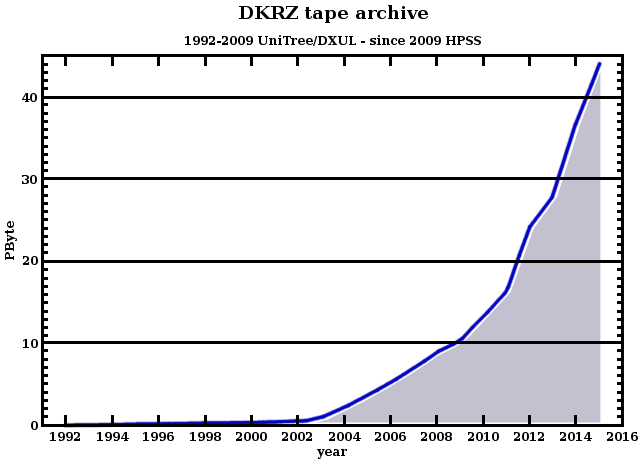
\includegraphics[width=0.9\linewidth]{DKRZ_data_growth.png}
	\caption{DKRZ data growth redrawn\\ citation needed}
	\label{fig:dkrz}
\end{wrapfigure}

\cref{fig:dkrz} illustrates the increasing data usage at the German Climate
Computing Center in Hamburg (DKRZ). Until now data compression at the DKRZ
already has been put to practise but "storage capacity does not grow as fast as
computation power" [citation needed]. Therefore optimizations regarding data
reduction are a reasonable method to minimize the need of upscaling existing
data archives.

\clearpage

\section{SCIL}

To further exploit the potential of lossy and lossless compression in research,
SCIL is being developed. SCIL is the Scientific Compression Interface
Library for the programming language C. Having conventional and specifically
developed compression algorithms integrated, it is able to compress data in
a variety of ways. After calling the program 'scil-config'\footnote{Not yet implemented}
to configure SCIL for the running platform, each compression can be customized
by providing parameters such as:

\bigskip

\begin{itemize}
	\item Absolute/Relative error tolerance
	\item Performance of compression in MB/s
	\item Dimensional layout of the data
\end{itemize}

\bigskip

Based on these parameters, the platform dependent configuration and the
characteristics of the data itself, SCIL will automatically choose the best
fitting compression algorithm at disposal\footnotemark[\value{footnote}].\par

\setcounter{footnote}{0}

\chapter{Design}
\label{Design}

\section{Problem Definition}

\bigskip

Many available compression algorithms perform different on distinct datasets.
Choosing the best algorithm for a given dataset is an assignment requiring
in depth knowledge of conventional compression methods. Furthermore it is
apparent that users are settling for one algorithm of their choice with which
they are compression various datasets. Algorithms performing better on some
datasets will be ignored compromising data reduction rates for consistency.\par
SCIL is a library which automates the task of algorithm choice while providing
a clean interface for compression and decompression. Its main goals are:

\bigskip

\begin{itemize}
	\item User friendliness
	\item Data adaptability
	\item Extensibility
	\item Platform independence
\end{itemize}

\bigskip

\clearpage

\section{Design Description}

\bigskip

At the core of SCIL there are the two essential methods to compress and
decompress data as well as a structure to hold the user specified compression
information. Calling the compression method invokes SCILs internal workflow in
which it chooses the best compression methods out of available algorithms.
The decision on which algorithm to choose is not only based on the users
parameter input but also on the data characteristics and the platform specific
configuration of SCIL. After writing the compressed buffer it is possible to
decompress again by simply calling the decompression method of SCIL.
In the following subsections a more detailed explaination of SCILs workflow
will be presented.

\bigskip

\subsection{Algorithm Decision}

\bigskip

After validating the parameters of the compress function call, it is determined
if the user explicitly forced to compress with a certain algorithm. In that case
the compression commences, providing relevant user specified parameters to the
chosen method. Otherwise the compression parameters are checked to determine
whether a lossless compression is needed (if the user provided no parameters on
error tolerance) or if a lossy compression method suffices the users needs. In
case of lossless compression the parameter restricting compression speed is
the only one consulted\footnote{Not yet implemented}. If none is given, SCIL
will default to best compression rates, regardless of compression speed. If the
user provided arguments describing error tolerance, SCIL considers lossy
algorithms, optionally with a subsequent lossless
compression\footnotemark[\value{footnote}]. In either case the platform specific
configuration of SCIL [see subsec ...] and current data characteristics are of
interest. Analizing the data for its characteristics is an optional
feature\footnotemark[\value{footnote}] as it can be very time consuming. Yet it
enables further customization of the compression by the user.

\setcounter{footnote}{0}

\clearpage

\subsection{Header Writing}

\bigskip

\renewcommand*{\thefootnote}{\arabic{footnote}}

The intermediate step between algorithm choice and actual compression is the
writing of meta data to the start of the compressed data buffer. This meta data
is often called header. The first byte in the header represents the algorithm
ID. Base on this number, SCIL is able to identify the correct decompression
method later on. The ID is the only part of the header guaranteed to be present.
Afterwards the datas dimensional layout will be written if the user chooses to
do so. Generally users are aware of the dimensional configuration of their data,
thus SCIL defaults to not storing it in the header\footnote{Currently always stores the dimensional configuration of the data}.
Nevertheless, storing the
dimensional layout in the header can be beneficial, for example if the data is
shared between users. At last, algorithm specific meta data is written. This
data is different from algorithm to algorithm and will be discussed in detail
in \cref{comp_data}.

\bigskip

\subsection{Compressing Data}
\label{comp_data}

\bigskip

At last, the actual compression of the data commences. Depending on the chosen
algorithm, compression rates and speeds can vary widely. Current Compression
Algorithms at disposal include:

\bigskip

\begin{itemize}
	\item memcpy \footnote{As the trivial compression for benchmarking puposes}
	\item abstol
	\item gzip
	\item sigbits
	\item fpzip
	\item zfp, absolute tolerance
\end{itemize}

\setcounter{footnote}{0}

\bigskip

The abstol and sigbits algorithms are specifically developed for SCIL. A
detailed description of their functionality can be found in \cref{abstol} and
\cref{sigbits} respectively. All other compression methods are included from
indepentent projects. A reference to those projects can be found in the
bibliography of this report.

\clearpage

\subsection{Decompressing Data}

\bigskip

The decompression of data is invoked by calling the designated function. Since
compression relevant data was stored in the header of the compressed buffer, the
user does not need to provide further information for decompression. Providing a
structure to hold dimensional data however is optional. If the user decided to
store the datas dimensional configuration at compression, this provided
structure will hold the dimensional configuration after decompression. If no
dimensional configuration was stored in the header of the compressed data, the
number of dimensions in the provided structure will be set to
zero\footnote{Not yet implemented}.

\setcounter{footnote}{0}

\chapter{Examples}

%In the following sections, example code is presented to illustrate the usage
%of SCIL. The example code is written in the programming language C and not in
%pseudo-code, due to SCIL currently being a pure C library.

\section{Compressing}

\bigskip

\begin{lstlisting}[caption=Compression with SCIL, label={lst:comp}]
// Providing user specified compression parameters
scil_hints hints;
hints.absolute_tolerance = 0.005;
hints.relative_tolerance_percent = 1.0;
hints.significant_bits = 5;
...

// Creating compression context
scil_context* context;
scil_create_compression_context(&context, &hints);

// Writing dimensional layout (1D, 100 elements)
size_t* lengths = (size_t*)malloc(sizeof(size_t));
lenghts[0] = 100;
scil_dims_t dimensions = scil_init_dims(1, lengths);

// Allocating destination and source buffer
double* source = (double*)malloc(100 * sizeof(double));
byte* destination = (byte*)malloc(100 * sizeof(double) + SCIL_BLOCK_HEADER_MAX_SIZE);

// Write data to source buffer
...

// Variable holding compressed buffer size after compression
size_t compressed_size;

// Compress data
scil_compress(SCIL_DOUBLE, destination, &compressed_size, source, dimensions, context);
\end{lstlisting}

\clearpage

\section{Decompressing}

\bigskip

\begin{lstlisting}[caption=Decompression with SCIL, label={lst:decomp}]

// Providing size of compressed buffer
size_t source_size = ... ;

// Providing structure for dimensional configuration
size_t* lengths = (size_t*)malloc(sizeof(size_t));
scil_dims_t dimensions = scil_init_dims(1, lengths);

// How many values are compressed in the source buffer
size_t element_count = 100;

// Allocating destination buffer
double* destination = (double*)malloc(element_count * sizeof(double));

// Decompressing
scil_decompress(SCIL_DOUBLE, destination, dimensions, source, source_size);
\end{lstlisting}

\chapter{Conclusion}
\label{Conclusion}

\section{Benchmarking}
Lorem ipsum dolor sit amet, consetetur sadipscing elitr, sed diam nonumy eirmod tempor invidunt ut labore et dolore magna aliquyam erat, sed diam voluptua.
At vero eos et accusam et justo duo dolores et ea rebum.
Stet clita kasd gubergren, no sea takimata sanctus est Lorem ipsum dolor sit amet.

\section{Final Words}

\bibliographystyle{alpha}
\bibliography{literatur}

\appendix
\appendixpage

\chapter{abstol}
\label{abstol}

Lorem ipsum dolor sit amet, consetetur sadipscing elitr, sed diam nonumy eirmod tempor invidunt ut labore et dolore magna aliquyam erat, sed diam voluptua.
At vero eos et accusam et justo duo dolores et ea rebum.
Stet clita kasd gubergren, no sea takimata sanctus est Lorem ipsum dolor sit amet.

\chapter{sigbits}
\label{sigbits}

\listoffigures

\lstlistoflistings

\listoftables

\chapter*{}

\thispagestyle{empty}

\section*{Eidesstattliche Versicherung}

\begin{otherlanguage}{ngerman}
Hiermit versichere ich an Eides statt, dass ich die vorliegende Arbeit im Studiengang XXX selbstständig verfasst und keine anderen als die angegebenen Hilfsmittel -- insbesondere keine im Quellenverzeichnis nicht benannten Internet-Quellen -- benutzt habe.
Alle Stellen, die wörtlich oder sinngemäß aus Veröffentlichungen entnommen wurden, sind als solche kenntlich gemacht.
Ich versichere weiterhin, dass ich die Arbeit vorher nicht in einem anderen Prüfungsverfahren eingereicht habe und die eingereichte schriftliche Fassung der auf dem elektronischen Speichermedium entspricht.

\bigskip

\noindent
Ich bin damit einverstanden, dass meine Abschlussarbeit in den Bestand der Fachbereichsbibliothek eingestellt wird.
\end{otherlanguage}

\bigskip
\bigskip
\bigskip

\begin{center}
\begin{tabular}{ll}
	\rule{0.35\textwidth}{0.4pt} & \rule{0.55\textwidth}{0.4pt} \\
	Ort, Datum & Unterschrift
\end{tabular}
\end{center}

\end{document}
